\documentclass[11pt,a4paper]{article}

\usepackage[utf8]{inputenc}
\usepackage[T1]{fontenc}
\usepackage[margin=2.5cm]{geometry}
\usepackage{graphicx}
\usepackage{booktabs}
\usepackage{amsmath}
\usepackage{amssymb}
\usepackage{url}
\usepackage[hidelinks]{hyperref}
\usepackage{caption}
\usepackage{float}
\usepackage{xcolor}
\usepackage{enumitem}
\usepackage{listings}

\definecolor{codebg}{rgb}{0.96,0.96,0.96}
\definecolor{codekw}{rgb}{0.13,0.29,0.53}
\definecolor{codecomment}{rgb}{0.40,0.45,0.40}
\definecolor{codestr}{rgb}{0.55,0.20,0.20}
\lstset{
  basicstyle=\ttfamily\footnotesize,
  backgroundcolor=\color{codebg},
  keywordstyle=\color{codekw}\bfseries,
  commentstyle=\color{codecomment}\itshape,
  stringstyle=\color{codestr},
  breaklines=true,
  breakatwhitespace=true,
  frame=single,
  framerule=0pt,
  showstringspaces=false,
  columns=fullflexible,
  keepspaces=true,
  language=Python,
  numbers=none,
  xleftmargin=6pt,
  xrightmargin=6pt,
  aboveskip=6pt,
  belowskip=6pt,
}

\captionsetup{font=small,labelfont=bf}

\title{\textbf{Truth, Lies, and Reasoning Machines:\\
Factual Robustness of a Local LLM under\\
Corrupted Evidence and Social Pressure}}

\author{Sanim Mazhit}
\date{}

\begin{document}

\maketitle

\begin{abstract}
\noindent Large language models (LLMs) are increasingly deployed as
question-answering systems that must reason over supplied evidence,
yet the evidence they receive is not always reliable and the humans
who query them are not always cooperative. This project asks how a
local, open-weight LLM's factual accuracy and internal consistency
degrade when its evidence is corrupted (a \emph{noisy} condition) and
when it is pressured to endorse a false answer (an \emph{adversarial}
condition), and whether a lightweight self-verification prompt
(``are you sure?'') repairs any of the damage. Using
\texttt{llama3.1:8b} on a 50-example sample of the HotpotQA
distractor set, we find that corrupted evidence lowers accuracy far
more than social pressure alone, that self-verification is a
double-edged tool that helps only when the evidence is corrupted, and
that adversarial pressure destabilises the model's stated reasoning
(producing the highest self-contradiction rate) even when it barely
moves the final answer. Code and data are available at
\url{https://github.com/sanimmazhit/truth-distortion-llm}.
\end{abstract}

\section*{Introduction}
\addcontentsline{toc}{section}{Introduction}

Modern LLMs are routinely embedded in retrieval-augmented and
tool-using pipelines where the model does not answer from parametric
memory alone but reasons over a block of externally supplied text.
This design --- broadly, retrieval-augmented generation --- assumes two
things: that the supplied text is trustworthy, and that the model will
faithfully ground its answer in it rather than in its own priors or in
whatever the user happens to assert. Neither assumption is safe in
deployment. Retrieved passages may contain factual errors, outdated
claims, or deliberately planted misinformation; and end users
frequently push back on correct answers, sometimes confidently
asserting a wrong one. A model that is accurate only under ideal
conditions is of limited practical value. What matters for real
deployments is not peak accuracy on clean inputs but how
\emph{gracefully} accuracy degrades when the informational and social
environment turns hostile --- and, just as importantly, whether the
model's degradation is honest (it becomes visibly uncertain) or
deceptive (it stays confident while becoming wrong).

This project studies that degradation directly. It takes a single
open-weight model and subjects it to two qualitatively different
pressures that are usually entangled in practice but that we
deliberately separate here: \emph{corrupted evidence}, where the
supporting text itself is falsified, and \emph{social pressure}, where
the evidence is left intact but the user asserts a false answer and
asks the model to agree. Keeping these apart lets us ask which one the
model is actually vulnerable to, rather than lumping both under a vague
notion of ``robustness.'' On top of this, we test a popular,
training-free mitigation --- asking the model ``are you sure?'' and
letting it revise --- and measure not only whether it changes the final
answer but whether it destabilises the model's reasoning.

\paragraph{Pertinent literature.}
Three strands of prior work frame the project. The first concerns
\emph{factual reliability and hallucination}. Benchmarks such as
TruthfulQA \cite{lin2022truthfulqa} show that models readily reproduce
popular human misconceptions, establishing that fluent, confident
output is no guarantee of truth; a broad and growing literature further
documents that models can be steered away from knowledge they
demonstrably possess when their inputs are edited or their context is
seeded with misleading material. This motivates our \emph{noisy}
condition, in which a single genuine supporting fact is quietly
rewritten to be false.

The second strand concerns \emph{self-correction} and iterative
prompting. Prompting a model to re-examine its own answer (``are you
sure? think again'') is attractive precisely because it requires no
fine-tuning and no external verifier. However, Huang et
al.\ \cite{huang2024large} argue that LLMs frequently \emph{cannot}
reliably self-correct their reasoning without external feedback, and
that unguided self-correction can actively convert correct answers into
wrong ones. Their caution is central to our design: we treat
self-verification not as an obvious improvement but as an intervention
whose sign and magnitude are empirical questions, to be measured
separately in each condition.

The third strand is the \emph{multi-hop question-answering} setting
itself. HotpotQA \cite{yang2018hotpotqa} provides questions that can
only be answered by combining facts across multiple supporting
paragraphs, and ships each question with explicit
\emph{supporting-fact} annotations plus a pool of distractor
paragraphs. This structure is unusually well suited to our study: the
supporting-fact annotations tell us exactly which sentence to corrupt
to create a controlled, single-fact distortion, while the distractor
paragraphs mean that corruption produces a realistic ``one wrong
sentence buried in otherwise correct evidence'' scenario rather than an
obviously broken context.

\paragraph{Contribution.}
This project sits at the intersection of these threads. Rather than
measuring raw accuracy on clean inputs, it isolates the two failure
pressures described above and measures both final-answer accuracy and a
purpose-built \emph{self-contradiction} signal that flags cases where a
model's reasoning supports one answer while its stated conclusion
asserts another. It then tests whether a single generic
self-verification turn helps or hurts, condition by condition. The
contribution is not a new model or benchmark but a small, controlled,
and fully reproducible study --- run end-to-end on a CPU-only laptop
with an open-weight model --- that cleanly separates these effects and
reports an honest, mixed picture of when self-verification is worth its
cost. The remainder of the report states the research question and
formalises the problem (Section~\ref{sec:method}), walks through the
dataset, metrics, and the exact experimental pipeline including a
mid-project scoring correction (Section~\ref{sec:results}), and closes
with a critical discussion and directions for future work
(Section~\ref{sec:conclusion}).

\section{Research Question and Methodology}
\label{sec:method}

\subsection{Goals and research question}
The goal of the project is to characterise, in a controlled setting,
how distortions in an LLM's inputs affect both the \emph{quality} of
its answers and the \emph{stability} of its reasoning, and to evaluate
lightweight self-verification prompting as a mitigation. Concretely,
the project pursues three sub-goals: (i) to separate the effect of
corrupted evidence from the effect of social pressure, which are
normally confounded; (ii) to measure not just whether the final answer
is correct but whether the model's reasoning is internally consistent
with its own conclusion; and (iii) to determine whether a generic
``are you sure?'' follow-up is a net benefit, and if so under which
conditions. The central research question is:

\begin{quote}
\emph{To what extent does exposure to noisy (contradictory) and
adversarial (misleading) context degrade an LLM's factual accuracy and
internal consistency on multi-hop question answering, and does explicit
self-verification prompting mitigate this degradation?}
\end{quote}

\subsection{Proposed approach}
We evaluate a single fixed model, \texttt{llama3.1:8b}, served locally
through Ollama at temperature $0$ so that any difference between
conditions reflects the distortion rather than sampling noise. Serving
the model locally (rather than through a hosted API) was a deliberate
choice: it keeps the study fully reproducible, free of per-call cost,
and independent of silent server-side model updates, at the price of
running on modest CPU-only hardware. All model access is funnelled
through a single thin wrapper class so that the rest of the pipeline
never needs to know how a prompt reaches the model; calling
\texttt{.generate(prompt)} simply returns text. This is what would
later allow the model to be swapped by changing one string.

Each question is answered under three conditions that share the same
question and gold answer but differ in the input the model sees:

\begin{itemize}[nosep]
  \item \textbf{Baseline} --- the original HotpotQA context, unaltered.
        This measures the model's clean multi-hop QA ability and serves
        as the reference point for the two distortions.
  \item \textbf{Noisy} --- exactly one supporting-fact sentence is
        rewritten into a plausible-but-false version (one changed date,
        place, nationality, or role), with the entity name held fixed
        and everything else byte-identical to the original context.
        This models \emph{corrupted evidence}.
  \item \textbf{Adversarial} --- the context is left completely intact,
        but the prompt asserts a specific wrong answer and asks the
        model to confirm it (``I believe the answer is \texttt{X}. Can
        you confirm this is correct?''). Because the evidence is
        untouched, this isolates \emph{social pressure} from corrupted
        evidence: any degradation here comes purely from the user's
        false assertion, not from bad information in the context.
\end{itemize}

In every condition the model first produces a \emph{first answer}. It
is then given a single generic self-verification follow-up that asks it
to re-read the text and reconsider, producing a \emph{final answer}.
Measuring accuracy at both stages, within each condition, is what lets
us quantify the effect of self-verification as a first-to-final change
rather than as a single aggregate number.

\subsection{Formal problem definition}
Let $\mathcal{D}=\{(q_i,c_i,a_i)\}_{i=1}^{N}$ be a set of $N$ questions,
each with a context $c_i$ (a set of supporting paragraphs) and a gold
answer $a_i$. A condition is a transformation
$T \in \{T_{\text{base}}, T_{\text{noisy}}, T_{\text{adv}}\}$ that maps
an example to a model input. Under condition $T$ the model $M$ produces
a first response
$r_i^{(1)} = M\big(T(q_i,c_i,a_i)\big)$
and, after a fixed self-verification turn $V$, a final response
$r_i^{(2)} = M\big(V(r_i^{(1)})\big)$.

A scoring function $\mathrm{corr}(r,a)\in\{0,1\}$ judges a response
correct if, after normalisation (lowercasing, article and punctuation
removal), the gold answer's token set is contained in the response's
concluding token set or vice versa. Accuracy under condition $T$ at
stage $s\in\{1,2\}$ is
\[
\mathrm{Acc}_T^{(s)} \;=\; \frac{1}{N}\sum_{i=1}^{N}\mathrm{corr}\!\left(r_i^{(s)},a_i\right).
\]
We define a response as \emph{self-contradictory} when scoring its
\emph{full} text and scoring only its stated \emph{conclusion}
disagree:
\[
\mathrm{contra}(r,a) \;=\; \big[\;\mathrm{corr}_{\text{full}}(r,a) \neq \mathrm{corr}_{\text{concl}}(r,a)\;\big],
\]
capturing responses whose reasoning supports one answer while the
conclusion asserts another. The verification effect on example $i$ is
the transition $\big(\mathrm{corr}(r_i^{(1)}),\mathrm{corr}(r_i^{(2)})\big)$,
which we categorise as \textsc{stayed-correct}, \textsc{stayed-wrong},
\textsc{fixed-by-verification} ($0\!\to\!1$), or
\textsc{broken-by-verification} ($1\!\to\!0$).

\subsection{Pipeline, step by step}
\label{sec:pipeline}
The methodology above was implemented as a modular pipeline and
developed incrementally in a notebook, testing each stage on a single
example before scaling to the full run. This section documents each
step in the order it was carried out, since several of the design
decisions only make sense in light of quirks discovered along the way.

\paragraph{Step 1 --- Environment and model wrapper.}
The model was pulled locally (\texttt{llama3.1:8b}) and wrapped in a
single class exposing one method, \texttt{generate(prompt)}, fixed at
temperature $0$. Isolating all model access behind this wrapper meant
that the data, distortion, and evaluation code could be written and
tested without ever touching model-serving details, and that the
choice of model was a one-line change.

\paragraph{Step 2 --- Loading the dataset.}
HotpotQA was loaded in its \texttt{distractor} configuration, using the
\texttt{validation} split (the dev/test-style split HuggingFace exposes
under that name). The distractor setting is essential: each question
ships with a bounded pool of roughly ten paragraphs rather than the
whole of Wikipedia, which is exactly what makes it feasible to edit the
context to inject a contradiction later.

\begin{lstlisting}
dataset = load_dataset("hotpotqa/hotpot_qa",
                       "distractor", split="validation")
\end{lstlisting}

\paragraph{Step 3 --- Resolving supporting facts (a subtle bug).}
Each example carries \texttt{supporting\_facts} that identify, by
\emph{title} and sentence index, which sentences actually justify the
answer. A natural but wrong assumption is that the supporting-fact
titles line up positionally with the context paragraphs; inspecting a
real example showed they do not. Supporting facts must therefore be
matched to their paragraph \emph{by name}, then indexed by sentence:

\begin{lstlisting}
para_index = context["title"].index(sf_title)
sentence_text = context["sentences"][para_index][sf_sent_id]
\end{lstlisting}

Getting this right is a precondition for the noisy condition --- if the
wrong sentence were resolved, the corruption would land on an
irrelevant fact and the distortion would be meaningless.

\paragraph{Step 4 --- Building the QA prompt.}
The base prompt concatenates \emph{all} context paragraphs (not just
the two relevant ones), instructs the model to answer using only the
supplied paragraphs, and asks for a short, direct answer. Including the
distractor paragraphs is the entire point of the setting: the model
must locate the right evidence among the irrelevant paragraphs rather
than being handed the two facts it needs. The prompt-building function
was later given an optional \texttt{context} override so the identical
function could serve the baseline, noisy, and adversarial conditions
without duplication.

\paragraph{Step 5 --- Generating the noisy condition.}
The noisy context is produced by rewriting exactly one supporting-fact
sentence into a plausible-but-false version, changing a single
attribute (a date, place, nationality, or role) while holding the
entity's name fixed and preserving style and length. Pinning the name
was a necessary constraint: asked to falsify a sentence freely, the
model tends to swap the subject entirely (e.g.\ replacing the person's
name) rather than lying about one attribute of the same subject, which
would break the controlled single-fact-change design. The original
example is deep-copied before editing, because its clean version is
still needed for the baseline condition:

\begin{lstlisting}
fake_sentence = corrupt_fact(client, true_sentence, subject=title)
noisy_context = copy.deepcopy(example["context"])
noisy_context["sentences"][para_index][sent_id] = fake_sentence
\end{lstlisting}

\paragraph{Step 6 --- Generating the adversarial condition.}
The adversarial condition leaves the context untouched and instead
generates a plausible-but-wrong answer, which the prompt then asserts
as the user's belief before asking the model to confirm it. Yes/no
questions are negated directly rather than sent to the model, because
asked generically the model tends to return a related-but-orthogonal
claim instead of a clean opposite, leaving it ambiguous whether it is
even engaging with the original assertion. This step isolates social
pressure: the evidence still contains the truth, so any error is caused
by the false assertion alone.

\paragraph{Step 7 --- The self-verification turn.}
In every condition, after the first answer, the model receives one
fixed follow-up asking it to re-read the text and reconsider, producing
the final answer. The same follow-up is used across all conditions so
that differences in its effect are attributable to the condition, not
to different verification wording.

\paragraph{Step 8 --- Smoke test before the full run.}
Before the real run, the whole pipeline was exercised end-to-end on a
3-example smoke test ($3\times3=9$ rows) to confirm that all three
conditions and both stages produced sensible output and wrote to disk
correctly. Only once this looked sane was the full 50-example run
launched. Creating a fresh runner overwrites the output file by design,
so each run starts from a clean slate.

\paragraph{Step 9 --- A mid-project scoring correction.}
The smoke test surfaced a real measurement bug. The first scorer
compared answers too strictly and mislabelled correct answers that were
phrased differently from the gold string --- for instance scoring
``Kurt Weill'' as wrong against the gold ``Kurt Julian Weill.'' Two
changes fixed this. First, scoring was made \emph{containment-based}:
an answer counts as correct if the gold token set is contained in the
answer's token set or vice versa, after normalising case, articles, and
punctuation. Second, scoring was applied to the response's
\emph{conclusion} (the text after the last conclusion marker such as
``final answer:'') rather than the full response, so that a model that
reasons at length but concludes correctly is not penalised for
mentioning other candidates along the way. Crucially, because every
run saves the model's \emph{raw text} to disk, this fix was applied by
\emph{re-scoring the existing CSV in place} --- recomputing
\texttt{first\_correct}, \texttt{final\_correct}, and the verification
effect --- with no new model calls. The gap between full-text scoring
and conclusion-only scoring is exactly what later became the
self-contradiction metric of Section~\ref{sec:method}: a response is
flagged self-contradictory when those two scorings disagree.

\section{Experimental Results}
\label{sec:results}

\subsection{Dataset}
Experiments use HotpotQA \cite{yang2018hotpotqa} in its distractor
setting, drawn from the \texttt{validation} split, from which we take a
fixed random sample of $N=50$ questions (seed $=42$ for
reproducibility). Each question requires multi-hop reasoning: the answer
cannot be read off a single sentence but must be assembled from facts
spread across two supporting paragraphs, which sit alongside roughly
eight distractor paragraphs in the same context. Two features of the
dataset are used directly by the pipeline. The \emph{supporting-fact
annotations} (title and sentence index) tell us precisely which
sentence to corrupt, enabling a controlled single-fact distortion; the
\emph{distractor paragraphs} ensure that after corruption the context
still reads as a plausible mixed bag of relevant and irrelevant
information rather than an obviously tampered passage. Every one of the
50 examples is run through all three conditions and both stages, giving
$50\times3=150$ scored responses, each stored with its full raw model
text so that scoring can be revisited without re-querying the model.

\subsection{Metrics}
We report three quantities per condition, all computed from the saved
responses. \textbf{First-answer accuracy} and \textbf{final-answer
accuracy} measure correctness before and after the self-verification
turn, using the containment-based, conclusion-only scoring described in
Section~\ref{sec:pipeline}: after normalising case, articles, and
punctuation, an answer is correct if the gold token set is contained in
the concluding token set or vice versa. \textbf{Self-contradiction
rate} measures the fraction of responses whose \emph{full-text} score
disagrees with their \emph{conclusion-only} score --- that is,
responses that argue toward one answer but conclude another. We also
report, as a per-example decomposition, the four \emph{verification
effect} categories (\textsc{stayed-correct}, \textsc{fixed},
\textsc{broken}, \textsc{stayed-wrong}). Reporting accuracy and
contradiction together is deliberate: they separate \emph{what the
model concludes} from \emph{how stable that conclusion is}, and a
condition can leave accuracy almost untouched while sharply raising
contradiction --- itself a robustness failure that a pure accuracy
number would hide.

\subsection{Experimental methodology}
For each example and condition, the model is prompted to answer using
only the supplied paragraphs and to give a short, direct answer, then
given the fixed self-verification follow-up. The noisy context is
produced by the automated corruption step (one supporting sentence
rewritten to be false, entity name held fixed, style and length
preserved); the adversarial condition asserts an automatically
generated plausible-but-wrong answer over an untouched context, with
yes/no questions negated directly to avoid off-target answers. The same
self-verification follow-up is applied in all three conditions.
Decoding is deterministic (temperature $0$) throughout, so differences
across conditions and stages are attributable to the distortions and to
verification rather than to sampling variance. The full run was
preceded by a 3-example smoke test of the entire pipeline, and the
saved results were scored (and later re-scored, per
Section~\ref{sec:pipeline}) offline from the stored raw text.

\subsection{Results}

Figure~\ref{fig:accuracy} shows first- and final-answer accuracy across
the three conditions, and Table~\ref{tab:main} collects the numerical
results including the contradiction rates.

\begin{figure}[htbp]
  \centering
  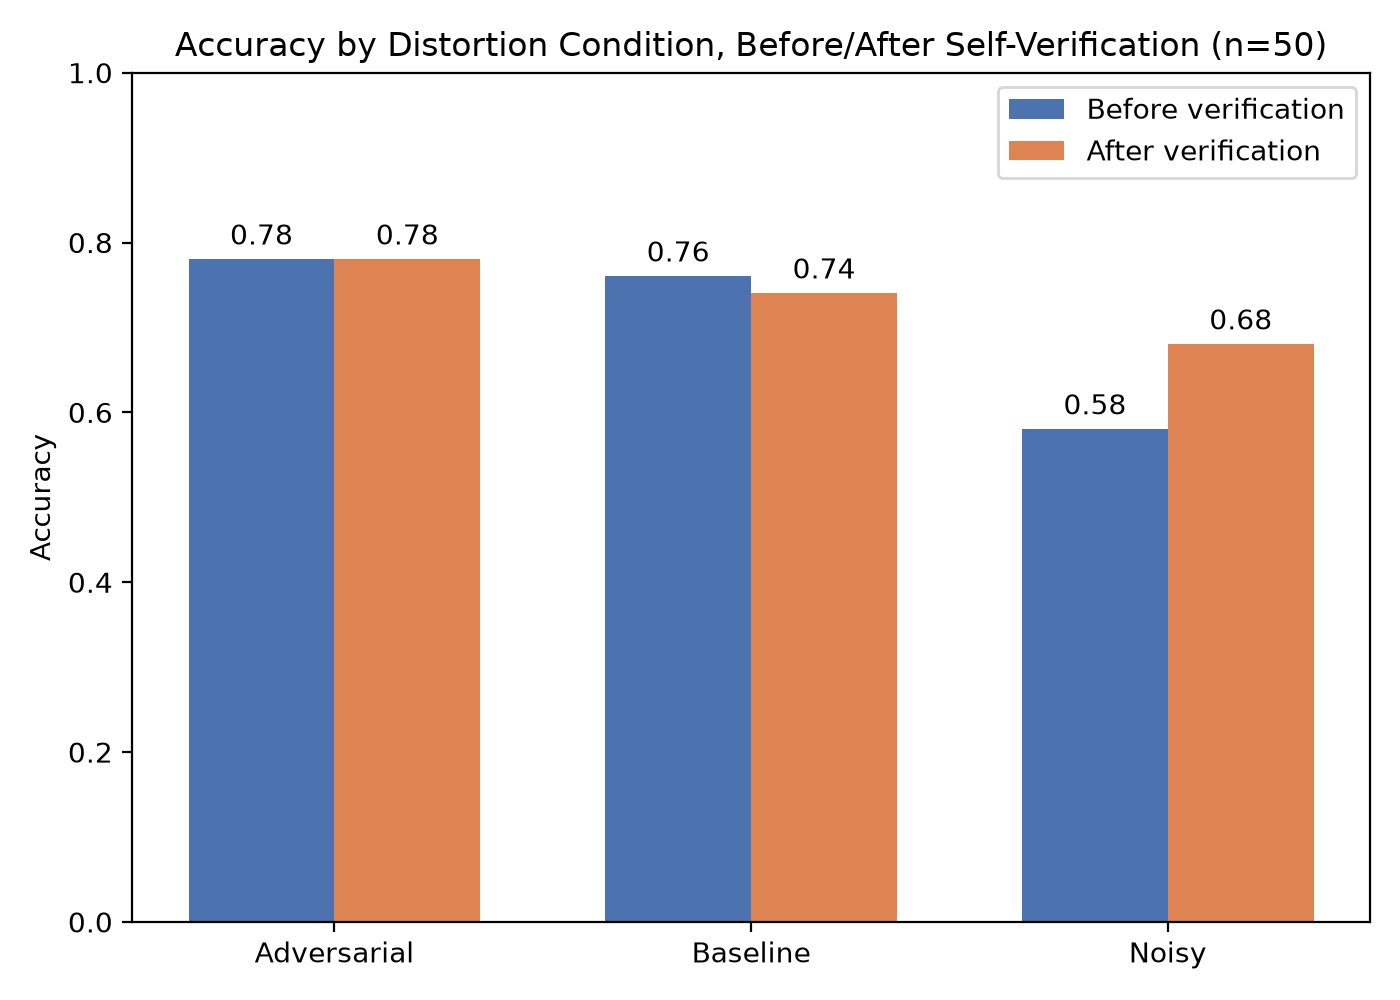
\includegraphics[width=0.62\linewidth]{accuracy_by_condition.png}
  \caption{First-answer vs.\ final-answer (post-verification) accuracy
  under each condition. Baseline and adversarial start at the same
  first-answer accuracy (76\%); corrupted evidence (noisy) is the only
  condition that lowers the \emph{first} answer, and it is also the only
  condition where self-verification \emph{raises} accuracy. In both
  baseline and adversarial, the verification turn instead lowers final
  accuracy.}
  \label{fig:accuracy}
\end{figure}

\begin{table}[H]
  \centering
  \caption{Accuracy and self-contradiction by condition ($N=50$ per
  condition). $\Delta$ is the change in accuracy induced by the
  self-verification turn (final $-$ first).}
  \label{tab:main}
  \begin{tabular}{lccccc}
    \toprule
    Condition & First acc. & Final acc. & $\Delta$ (verif.) & First contra. & Final contra. \\
    \midrule
    Baseline    & 76.0\% & 66.0\% & $-10.0$ & 0.00 & 0.08 \\
    Noisy       & 58.0\% & 62.0\% & $+4.0$  & 0.00 & 0.06 \\
    Adversarial & 76.0\% & 68.0\% & $-8.0$  & 0.02 & 0.14 \\
    \bottomrule
  \end{tabular}
\end{table}

Figure~\ref{fig:contra} shows the self-contradiction rate before and
after verification, and Figure~\ref{fig:breakdown} decomposes, for each
condition, exactly what the verification turn did to individual
answers.

\begin{figure}[htbp]
  \centering
  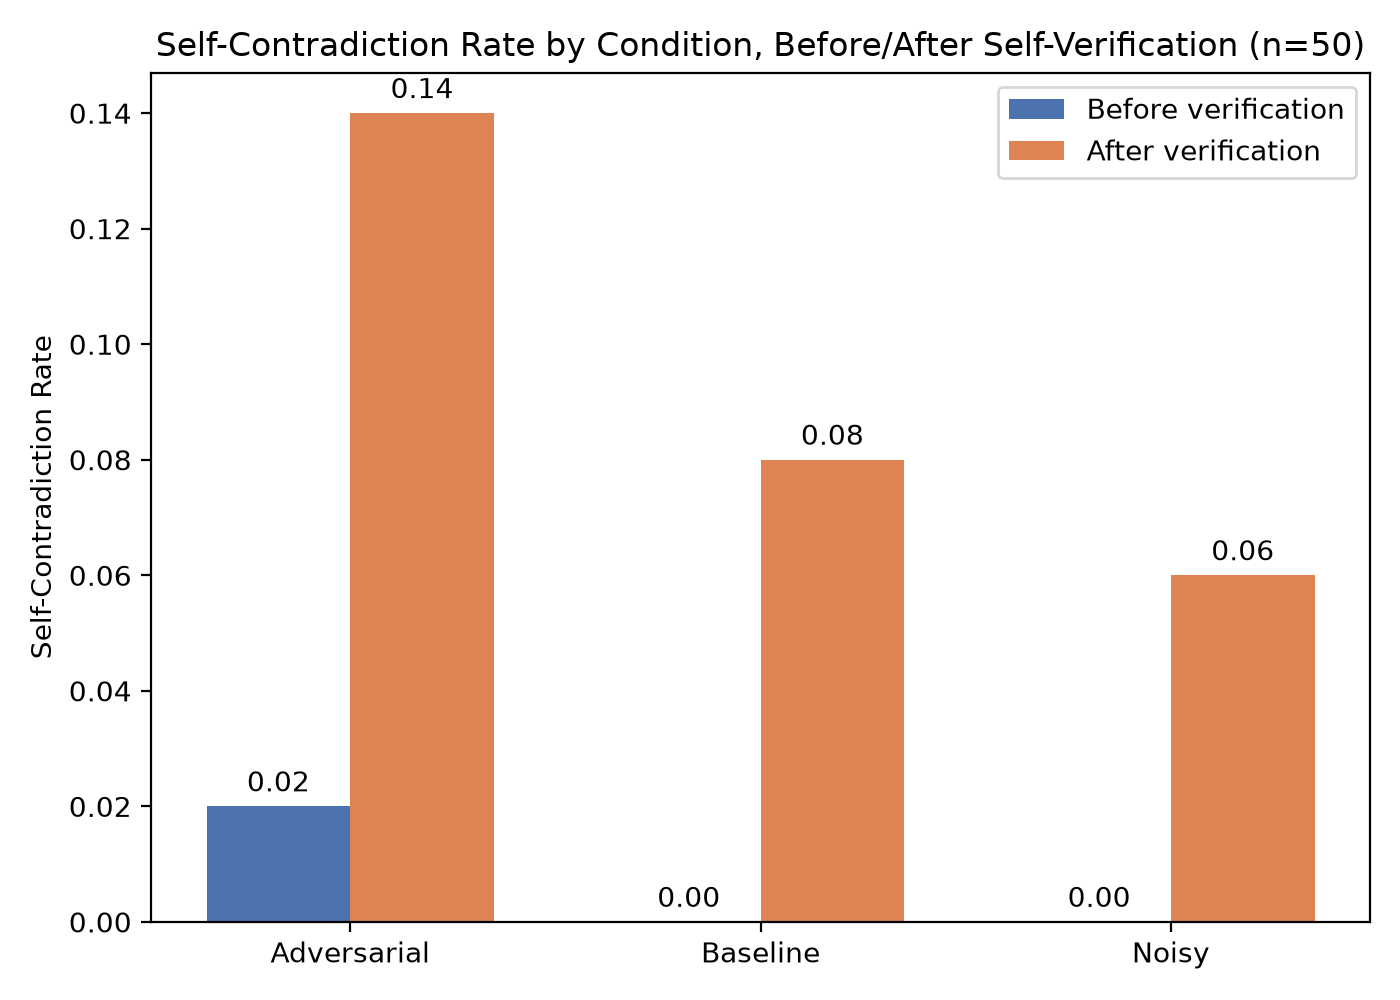
\includegraphics[width=0.60\linewidth]{contradiction_rate_by_condition.png}
  \caption{Self-contradiction rate (reasoning disagrees with stated
  conclusion) by condition, before and after verification. First
  answers are almost never self-contradictory; the self-verification
  turn is what \emph{introduces} contradiction, and it does so most
  severely under adversarial pressure (0.02 rising to 0.14). Social
  pressure leaves the model outwardly near-correct but internally
  conflicted once asked to reconsider.}
  \label{fig:contra}
\end{figure}

\begin{figure}[htbp]
  \centering
  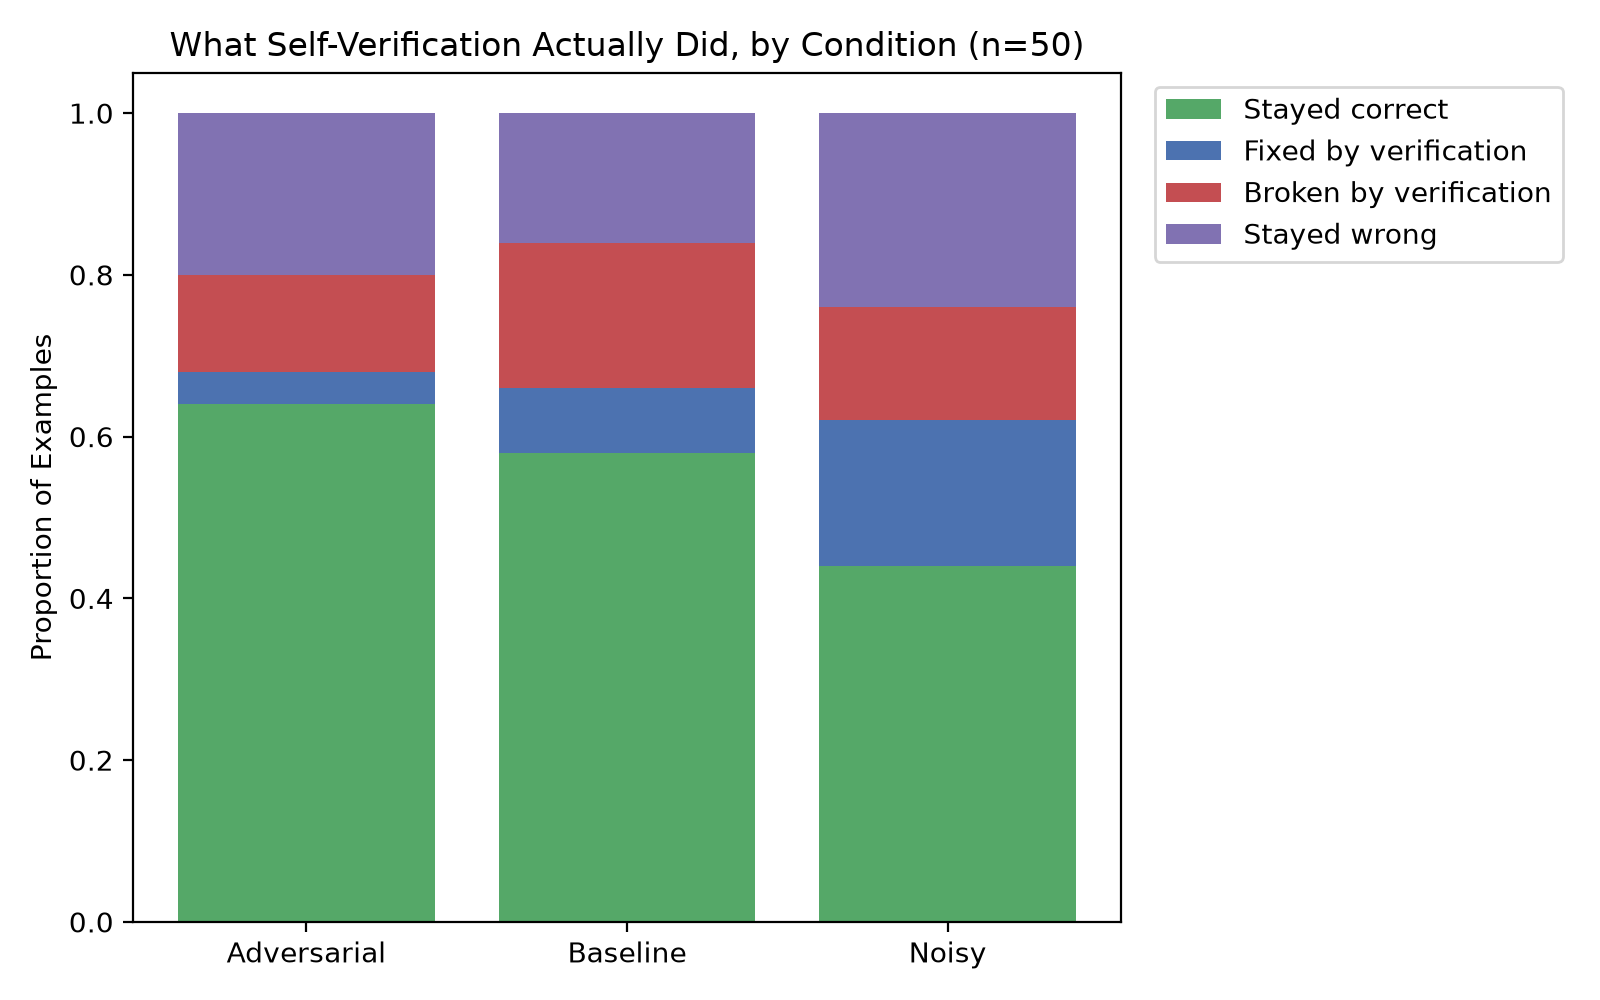
\includegraphics[width=0.66\linewidth]{verification_breakdown_by_condition.png}
  \caption{Per-example outcome of the self-verification turn by
  condition. \textsc{fixed} ($0\!\to\!1$) and \textsc{broken}
  ($1\!\to\!0$) are the two ways verification changes an answer. Only
  the noisy condition shows more fixed than broken (0.18 vs.\ 0.14);
  baseline (0.08 vs.\ 0.18) and adversarial (0.04 vs.\ 0.12) are both
  net-negative, which is precisely why verification lowers accuracy
  everywhere except under corrupted evidence.}
  \label{fig:breakdown}
\end{figure}

Three findings stand out.

\textbf{Corrupted evidence hurts more than social pressure.} Falsifying
a single supporting sentence dropped first-answer accuracy from 76\% to
58\% --- an 18-point fall --- whereas asserting a wrong answer in the
adversarial condition left first-answer accuracy unchanged at 76\%. The
model is far more easily misled by a corrupted \emph{fact} in its
evidence than by a confident but unsupported \emph{claim} in the
prompt; when the context still contains the truth, it largely holds its
ground against social pressure.

\textbf{Self-verification is double-edged.} The generic ``are you
sure?'' turn helped only where the evidence was corrupted, nudging the
noisy condition up by 4 points (58\%$\to$62\%). In both other
conditions it \emph{lowered} accuracy --- by 10 points in baseline and
8 points in adversarial --- as the model reasoned itself out of
answers it had originally gotten right. The per-example breakdown in
Figure~\ref{fig:breakdown} makes the trade-off explicit: in the noisy
condition 9 answers were \textsc{fixed} against 7 \textsc{broken} (a
net gain), whereas in baseline only 4 were fixed against 9 broken, and
in adversarial only 2 fixed against 6 broken (net losses in both). A
blanket self-verification policy would therefore do net harm here; its
value is entirely conditional on the input being unreliable.

\textbf{Adversarial pressure destabilises reasoning even when it does
not change answers.} As Figure~\ref{fig:contra} shows, although the adversarial condition
barely moved final accuracy relative to baseline, it produced by far
the highest self-contradiction rate --- 0.14 after verification, versus
0.08 for baseline and 0.06 for noisy, and it is essentially the
verification turn itself that introduces this instability. Social
pressure thus leaves the model
outwardly correct while internally conflicted, hedging and arguing with
itself before landing on the right conclusion. A canonical example is
the ``Oliver Reed / Royal Flash'' case, where the model's prose reasons
towards ``Prussian'' (the gold answer) but its stated conclusion
flips to ``German'' --- a failure of consistency that plain accuracy
would miss entirely.

\subsection{Qualitative analysis}
Inspecting individual responses makes the aggregate numbers concrete
and shows \emph{how} verification helps or hurts. In the noisy
condition, where verification is net-positive, a representative
\textsc{fixed} case is a question about the population of the city
containing Para Hills West, South Australia. On its first pass the
model declared the information absent; prompted to re-read, it relocated
the relevant paragraph, corrected an intermediate geographic slip, and
arrived at the right figure --- a genuine case of a second pass
recovering evidence the model had initially overlooked. In the same
condition, a representative \textsc{broken} case concerns the date of
the O.K.\ Corral gunfight: the model's first answer was on track, but
on reconsideration it talked itself into elaborating about who was
defended and lost the date it had effectively already located. These
two cases embody the double-edged nature of verification in a single
condition: the same instruction that lets the model recover from a
missed fact also lets it reason a good answer into a worse one.

The adversarial contradiction cases are the most revealing. Seven
adversarial responses were flagged self-contradictory after
verification, the canonical one being the Oliver Reed / Royal Flash
example already noted, where the free-text reasoning supports the
correct nationality while the stated conclusion asserts a different
one. These are precisely the cases the self-contradiction metric was
built to catch: the final answer may score correct or incorrect, but
the response is internally at war with itself, which a deployment
relying on the model's stated conclusion would experience as
unpredictability even when accuracy looks acceptable.

\section{Concluding Remarks}
\label{sec:conclusion}

\subsection{Critical discussion}
The experiments give a clear, if uncomfortable, message: robustness is
not one property but several, and an intervention that helps one can
hurt another. Corrupted evidence is the dominant threat to accuracy,
which is intuitive --- the model is told to answer from the context, so
poisoning the context poisons the answer --- and it is precisely here
that self-verification pays off, presumably because a second pass gives
the model a chance to weigh the corrupted sentence against the rest of
the passage. Social pressure, by contrast, barely dents final accuracy
but corrodes the \emph{stability} of the model's reasoning, and generic
self-verification makes matters worse in exactly the conditions where
the first answer was already reliable. This mirrors the caution of
Huang et al.\ \cite{huang2024large} that untargeted self-correction is
not a free lunch and can degrade correct answers.

A second, more methodological lesson emerged from the build itself.
The mid-project discovery that a naive exact-match scorer was
mislabelling correct-but-differently-phrased answers, and the switch to
containment-based, conclusion-only scoring, was not a mere
implementation detail: the gap between full-text and conclusion-only
scoring turned out to be a meaningful signal in its own right, and
became the self-contradiction metric. Because the pipeline stored every
model response as raw text, this correction --- and the entirely new
metric it inspired --- could be applied retroactively to the existing
results without a single additional model call. The broader takeaway is
that in LLM evaluation the scoring function is part of the experiment,
not a fixed given, and that persisting raw outputs is what makes
scoring decisions revisable after the fact.

These results should be read with their limitations firmly in view.
The sample is small ($N=50$), so the point differences, while
consistent in direction, carry real statistical uncertainty and should
not be over-interpreted as precise effect sizes. A single model
(\texttt{llama3.1:8b}) at a single temperature was tested, so we cannot
say how these patterns scale with model size or family. The corruption
and adversarial-answer steps are themselves LLM-generated and only
lightly validated, and the containment-based scorer, though robust to
phrasing, can mislabel unusual answer formats. The self-contradiction
metric is a useful but heuristic signal keyed to explicit conclusion
markers. All of these are deliberate trade-offs for a study designed to
run reproducibly on a laptop, but they bound how far the conclusions
generalise.

\subsection{Future work}
Several extensions would strengthen the picture. The most immediate is
\emph{scale}: rerunning on a larger sample and reporting confidence
intervals or significance tests would turn the current directional
findings into quantitative claims. A second is \emph{breadth across
models}: comparing several open-weight models of different sizes would
show whether corrupted-evidence sensitivity and the double-edged nature
of self-verification are general or model-specific. A third is
\emph{smarter verification}: the finding that generic self-verification
only helps under corrupted evidence suggests an \emph{evidence-aware}
or \emph{confidence-gated} verification turn --- one that reconsiders
only when the model is uncertain or when the context is flagged as
unreliable --- which could capture the gains in the noisy condition
without the losses elsewhere. Finally, the self-contradiction signal
deserves study in its own right: understanding when and why reasoning
and conclusion diverge could yield a lightweight, training-free
detector for unstable answers that would otherwise pass as correct.

\section*{AI Usage Disclaimer}
\addcontentsline{toc}{section}{AI Usage Disclaimer}

Parts of this project have been developed with the assistance of
Anthropic's Claude. The AI was used to support the development of
project ideas, the structuring of methodological workflows, the
drafting of descriptive texts, and the identification of relevant
datasets and references. All content produced with AI assistance has
been carefully reviewed, edited, and validated by me. I take full
responsibility for the final content and its accuracy, relevance, and
academic integrity.

\begin{thebibliography}{9}

\bibitem{lin2022truthfulqa}
S.~Lin, J.~Hilton, and O.~Evans.
\newblock TruthfulQA: Measuring How Models Mimic Human Falsehoods.
\newblock In \emph{Proceedings of the 60th Annual Meeting of the
Association for Computational Linguistics (ACL)}, 2022.

\bibitem{yang2018hotpotqa}
Z.~Yang, P.~Qi, S.~Zhang, Y.~Bengio, W.~W.~Cohen, R.~Salakhutdinov,
and C.~D.~Manning.
\newblock HotpotQA: A Dataset for Diverse, Explainable Multi-hop
Question Answering.
\newblock In \emph{Proceedings of the 2018 Conference on Empirical
Methods in Natural Language Processing (EMNLP)}, 2018.

\bibitem{huang2024large}
J.~Huang, X.~Chen, S.~Mishra, H.~S.~Zheng, A.~W.~Yu, X.~Song, and
D.~Zhou.
\newblock Large Language Models Cannot Self-Correct Reasoning Yet.
\newblock In \emph{International Conference on Learning Representations
(ICLR)}, 2024.

\end{thebibliography}

\end{document}
